\subsection{Inleiding}
De Satellite heeft verschillende communicatie middelen, onderanderen ethernet, CAN Bus en serieel communicatie. Alle deze vormen van communicatie moeten voldoen aan het volgende deelvraag: \textbf{Hoe kan er een robuuste communicatie gecreëerd worden tussen het hoofdsysteem en Satellite?}. Er moet gekeken worden hoe dit stabiel en robuust gedaan kan worden.

\subsection{Ethernet}
Satellite heeft standaard ethernet support dit betekent dat via een ethernet kabel naar een end device gecommuniceerd kan worden. Dit wordt alleen via de User Datagram Protocol (UDP) internet protocol gedaan. UDP is een standaard methode om data te versturen tussen twee systemen \autocite{CloudFlareUDP}. \newline

\noindent Om een betrouwbare communicatie te creëren zal er gebruikt gemaakt worden van een library. Een eigen library hiervoor te schrijven zal veel tijd kosten en is buiten het scoop van het project. Hiervoor zijn er een aantal opties om uit te kiezen: lwIP, uIP, FreeRTOS TCP/IP. Voor deze drie libraries wordt er gekeken wat de pluspunten en negatieve punten zijn:

\subsubsection{LWiP}
LWip (Lightweight TCP/IP) is een open source implementatie van TCP/IP stack dat zicht focust minder geheugen te gebruiken, maar nog steeds alle grote features te hebben. lwIP zorgt ervoor dat er makkelijk connectie gemaakt kan worden tussen verschillende systemen \autocite{LWIP}. Hieronder is een overzicht gemaakt \ref{tab:lwipoverzicht} met de pluspunten en de negatieve punten van LwIP.

\begin{table}[h!]
	\caption{Pluspunten en minpunten van LwIP}
	\begin{tabular}{p{8cm}p{8cm}}
	\toprule
	Pluspunten & Minpunten \\ \midrule
	Een kleine TCP/IP implementatie	met snelle performance. \autocite{lwipuip}	&  Niet geschikt voor hele kleine embedded systemen \autocite{lwipuip}         \\
																				&           \\
			   																	&           \\
			   																	&           \\ \bottomrule
	\end{tabular}
	
	\label{tab:lwipoverzicht}
\end{table}

\newpage
\subsubsection{UIP}
Hieronder is een overzicht \ref{tab:uipoverzicht} van de pluspunten en minpunten van UIP.
\begin{table}[h!]
	\caption{Pluspunten en minpunten van UIP}
	\begin{tabular}{p{8cm}p{8cm}}
	\toprule
	Pluspunten & Minpunten \\ \midrule
	Ontwikkelt voor systemen met echte beperkte snelheiden en geheugen \autocite{lwipuip} &           \\
			   															&           \\
			   															&           \\
			   															&           \\ \bottomrule
	\end{tabular}
	
	\label{tab:uipoverzicht}
\end{table}

\subsubsection{Conclusie}

\newpage
\subsection{CAN communicatie}
CAN is een groot onderdeel van de Sensor Maritime infrastructuur. De CAN communicatie wordt gebruik om te kunnen communiceren met het hoofdsysteem genaamd het hub. Hiervoor wordt een master en slave configuratie gebruikt. Het hub is de master en de Satellite en andere eindsystemen zullen dan de slave zijn. De master bepaalt hoe een slave apparaat zich gaat gedragen. CAN staat voor controlled area network, en maakt gebruik van een broadcast systeem. Dit betekent dat alle eindsystemen alle berichten ontvangen, De master kan niet specifiek naar een slave data sturen \autocite{can}. \newline

\noindent Sensor Maritime heeft een eigen protocol ontwikkeld wat gebouwd is op het CAN Bus. Dit zal deels aangepast moeten worden om de Satellite sensoren te kunnen ondersteunen. De huidige protocol wat gebruikt wordt is in afbeelding \ref{fig:canprotocol} te zien. Het protocol is opgebouwd uit blokjes wat uit 1 of 2 bytes bestaat. In tabel \ref{tab:cansensorprotocol} wordt beschreven wat de taak is van het blokje. 
\begin{figure}[h!]
	\label{fig:canprotocol}
	\caption{Sensor Maritime CAN protocol}
	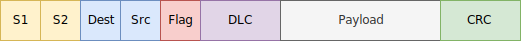
\includegraphics[width=\linewidth]{voorstudie/communicatie/can.png}
\end{figure}

\begin{table}[h!]
	\caption{Sensor Maritime CAN protocol opbouw}
	\label{tab:cansensorprotocol}
	\begin{tabular}{p{1.5cm}p{10.5cm}p{3cm}}
	\toprule
	\textbf{Blok} & \textbf{Beschrijving} & \textbf{Waarde}\\ \midrule
	S1		& Het eerst start byte, dit geeft het start aan van het CAN bericht en wordt gebruikt voor herkenning, dit is een vaste waard.	& 0x40 \\
	S2		& Het tweede start byte, dit geeft het start aan van het CAN bericht en wordt gebruikt voor herkenning, dit is een vaste waard. & 0x02 \\
	Dest	& Deze byte beschrijft voor wie het bericht bedoeld is.		& Verschillend per apparaat. \\
	Src		& Deze byte beschrijft van welke apparaat het bericht komt	& Verschillend per apparaat.\\ 
	Flag	& Dit geeft aan wat voor type bericht het is.             & 0 voor commando \\ 
			& & 1 voor request \\ 
	DLC		& DLC is een afkorting voor Data Length Code.             & \\ 
	Payload	& De data die aan de hand de flag. & Verschillend per bericht\\
	CRC		& CRC staat voor Cyclic redundancy check, dit beschrijft hoe groot het bericht is wat verstuurd word, Hiermee kan de ontvanger valideren of het juiste is ontvangen. & Verschillend per bericht\\ \bottomrule
	\end{tabular}
\end{table}

\subsubsection{Probleemstelling}
Om het volgende deelvraag te kunnen beantwoorden zal er een aanpassing gemaakt moeten worden aan de bestaande CAN protocol van Sensor Maritime. De deelvraag wat beantwoord moet worden luid als volgt \textbf{Hoe kan er een robuuste  communicatie gecreëerd worden tussen het hoofdsysteem en Satellite?}